\clearpage{}
\section{Ref types invite large refactorisation exercises}
\label{intro:ref-types}
SML obstinately supports destructive update, though its use is restricted to arrays and to data structures that incorporate the special $\iRef$ type. The following functions are used to program with $\iRef$. We use Haskell syntax for consistency.

\code{
	$\inewRef$   & $:: a     \to \iRef \ a$		\\
	$\ireadRef$  & $:: \iRef \ a \to a$		\\
	$\iwriteRef$ & $:: \iRef \ a \to a \to ()$	\\

}

$\inewRef$ takes an object and returns a fresh mutable reference to that object. $\ireadRef$ takes a reference to an object and returns the object. $\iwriteRef$ takes a mutable reference, a new object, and updates the reference to point to the new object.

Although serviceable, tying update to a particular type constructor forces the programmer to decide which parts of their structures should be updatable when their types are defined. On the surface this may seem reasonable, but consider the design of a simple library for a cons-list. We start with the data type:

\code{
	\mc{2}{$\kdata \ \iList \ a$}	\\
		& $= 		\iNil$ 		\\
		& $\ \mid 	\iCons \ a \ (\iList \ a)$
}

We would now like to define a set of functions which operate on values of this type. One such function is $\iindex$, which returns the element at a particular position in the list:

\code{
	\mc{3}{$\iindex :: \iInt \to \iList \ a \to a$}				\\
	$\iindex \ 0$	& $(\iCons \ x \ixs)$	& $ = x$			\\
	$\iindex \ n$  	& $(\iCons \ x \ixs)$  	& $ = \iindex \ (n-1) \ \ixs$	\\
	$\iindex \ \_ $ & $\iNil$          	& $ = \ierror \ \dots$
}

Suppose that once we have finished this definition we then want a function $\ireplace$ that destructively replaces the element at a certain position in the list. This requires the head of the $\iCons$ cell to be updatable, so we insert a $\iRef$ constructor into the data type:

\code{
	\mc{3}{$\kdata \ \iList \ a$}					\\
		& $= 		\iNil$					\\
		& $\ \mid	\iCons \ (\iRef \ a) \ (\iList \ a)$
}

The definition of $\ireplace$ is then:

\code{
	$\ireplace \ 0 \ e \ (\iCons \ \irx \ \ixs)$	
		& $= \iwriteRef \ \irx \ e $	\\
	$\ireplace \ n \ e \ (\iCons \ \irx \ \ixs)$
		& $= \ireplace \ (n-1) \ e \ \ixs$
}

This is all well and good, but as the $\iList$ type has changed we need to go back and change the definition of $\iindex$ to read the element out of the reference before returning it. We must also inspect every other function we've defined that uses the $\iList$ type. If a function accesses the head of a $\iCons$ cell then it needs a call to $\ireadRef$ as well.

\code{
	\mc{3}{$\iindex :: \iInt \to \iList a \to a$}				\\
    	$\iindex \ 0 \ (\iCons \ x \ \ixs)$	& $= \ireadRef \ x$		\\
    	$\iindex \ n \ (\iCons \ x \ \ixs)$	& $= \iindex \ (n-1) \ \ixs$	\\
    	$\iindex \ \_ \ \iNil$			& $= \ierror \ \dots$		
}


Conceptually, the operation of $\iindex$ hasn't changed at all. $\iindex$ still recursively steps through the list until it finds the desired element, then returns it. However, we had to modify its definition because we added a function to the library which requires a certain property (mutability) of the data structure, even though $\iindex$ itself doesn't make use of that property. Notice that the modifications required are purely mechanical in nature, and that this problem is very similar to monad creep discussed in the previous section.

Suppose that after defining a few more functions, we desire a new one called $\iinsertAt$. This function will make use of destructive update to insert a new element at a particular position in the list. This requires the $\itail$ of each $\iCons$ cell to be mutable as well, so we have to change the data type once again:

\code{
	\mc{2}{$\kdata \ \iList \ a$}	\\
		& $= \ \iNil$		\\
		& $\ \mid \ \iCons \ (\iRef \ a) \ (\iRef \ (\iList \ a))$
}

The definition for $\iinsertAt$ is:

\code{
	\mc{3}{$\iinsertAt :: \iInt \to a \to \iList \ a \to ()$}					
	\\[1ex]
	\mc{3}{$\iinsertAt \ \_ \ e \ \iNil \ \ \ = \ierror \dots$}
	\\[1ex]
	\mc{3}{$\iinsertAt \ 0  \ e \ (\iCons \ r \ \irxs)$} 						\\
		& $\ =$	& \mc{2}{$\klet \  \ixs = \ireadRef \ \irxs$}					\\
		&	& \mc{2}{$\kin \ \ \iwriteRef \ \irxs \ (\iCons \ (\iRef \ e) \ (\iRef \ixs))$}
	\\[1ex]
	\mc{3}{$\iinsertAt \ n \ e \ (\iCons \ r \ \irxs)$}						\\
		& $\ =$ & \mc{2}{$\klet \  \ixs = \ireadRef \ \irxs$}					\\
		&	& \mc{2}{$\kin \ \ \iinsertAt \ (n-1) \ e \ \ixs$}		
}

Once again, we must go back and inspect every function we have defined so far to make sure that all accesses to the tail of a $\iCons$ cell first read the reference. Our $\iindex$ function is now:

\code{
	\mc{2}{$\iindex :: \iInt \to \iList \ a \to a$}	\\	
	$\iindex \ 0  \ (\iCons \ x \ \ixs)$	& $= \ireadRef \ x$	\\
	$\iindex \ n  \ (\iCons \ x \ \ixs)$ 	& $= \iindex \ (n-1) \ (\ireadRef \ xs)$	\\
	$\iindex \ \_ \ \iNil$		        & $= \ierror \ \dots$
}

More mechanical modifications have wasted more programming time. What can be done to alleviate this problem? The central activity of programming is defining data structures and writing functions which operate on them. Unless a programmer is simply replicating a program they have written before then they are unlikely to know exactly which parts of their structure should be wrapped in $\iRef$ and which can be left bare.

If we define all structures to be mutable from the start then we can avoid having to re-inspect existing functions as the data type evolves, though this would require many superfluous calls to $\ireadRef$. In addition, a naive implementation of $\iRef$ would simply insert reference objects into the run-time data structure, so we would pay a performance penalty as well:

\begin{center}
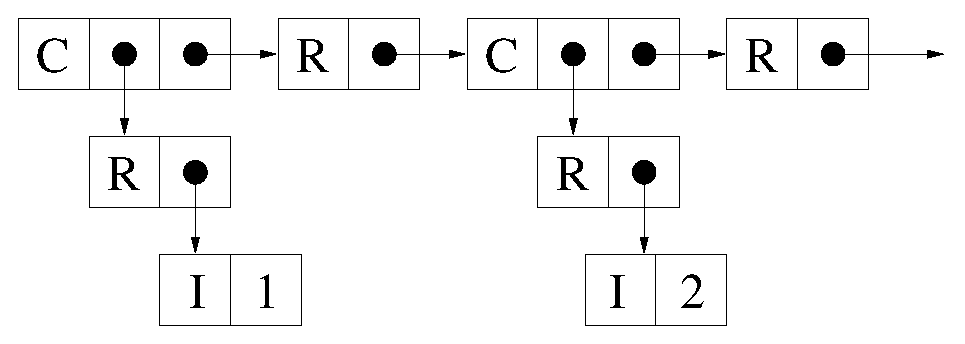
\includegraphics[scale=0.5]{1-Introduction/fig/ref-types/ref-list}
\end{center}

On the other hand, if we define our data types \emph{without} using $\iRef$, then structures of that type can not be updated --- ever. If those structures are provided by a library and a client programmer decides they actually \emph{do} want to perform an update, then it is likely that the only practical solution will be to define their own types and write code that duplicates functionality already present in the original library.

This is exactly the case with SML lists and tuples, which are all immutable. Although some code duplication can be alleviated by using similar module signatures for mutable and immutable objects, the fact that the two have fundamentally different types only serves to encourage it. If only the immutable versions are provided in base libraries, then users are encouraged to use these structures in cases where a mutable one would be more appropriate. This in turn relegates mutable structures to be second class citizens of the language.
